\documentclass[tikz,border=10pt]{standalone}
\usepackage{tikz}
\input{Core Tikz Library/colours}
\usetikzlibrary{angles,quotes,calc, intersections}
\usepackage{tkz-euclide} %for right angle marker

\begin{document}
\begin{tikzpicture}

    % Define the center of the circle
    \coordinate (O) at (0,0);
    
    % Draw the circle
    \draw[fill=lightGreen] (O) circle (2cm);
    \fill[black] (O) circle (2pt);

    % Place points B and D on the circumference
    % The angle for B is -75 degrees (150/2) and for D is 75 degrees
    \coordinate (D) at ($(O) + (-45:2cm)$);
    \coordinate (B) at ($(O) + (100:2cm)$);

    % Draw tangents from points B and D
    % Calculate tangent points
    \coordinate (T1) at ($(D)!4!-90:(O)$);
    \coordinate (T2) at ($(B)!4!90:(O)$);

    %extend tangents
    \coordinate (E1) at ($(D)!1!90:(O)$);
    \draw (D) -- (E1);
    \coordinate (E2) at ($(B)!1!-90:(O)$);
    \draw (B) -- (E2);
    % Find intersection point C
    \path [name path=line1] (B) -- (T2);
    \path [name path=line2] (D) -- (T1);
    \path [name intersections={of=line1 and line2,by={C}}];

    % Draw tangent lines
    \draw (B) -- (C) -- (D);
    
    %label lenghth ticks
    \tkzMarkSegment[pos=.5,mark=|](B,C);
    \tkzMarkSegment[pos=.5,mark=|](C,D);

    % Draw lines
    \draw (O) -- (B);
    \draw (O) -- (D);
    \draw (O) -- (C);

    %Mark angles
    \pic [draw, angle eccentricity=1.4, angle radius = 1cm] {angle = B--C--D};
    %marking right angles
    \tkzMarkRightAngle[size=.3](O,B,C);
    \tkzMarkRightAngle[size=.3](C,D,O);
    

\end{tikzpicture}

%2
\begin{tikzpicture}[scale=2]
    
        \coordinate (B) at (140:1);
        \coordinate (A) at (220:1);
        \coordinate (E) at (250:1);
        \coordinate (F) at (320:1);
        \draw[name path=circ, fill = pink!10] (0,0) circle (1);
        \path[name path=BD] (B) -- ($(B)!2!65:(A)$);
        \path[name path=AC] (A) -- ($(A)!1.5!-30:(B)$);
        \path[name intersections={of=circ and BD, by={[]K,D}}];
        \path[name intersections={of=AC and circ, by={C}}];
        \draw[color = pink!60, thick, line join=bevel] (A) -- (B) -- (D) -- (C) -- cycle;
        \draw[color =primaryGreen, thick, line join=bevel] (A) -- (E) -- (D) -- (F) -- cycle;

        \pic [draw, color=pink, "b", angle eccentricity=1.4, angle radius = 0.5cm] {angle = A--B--D};
        \pic [draw, color=primaryGreen, "a", angle eccentricity=1.4, angle radius = 0.3cm] {angle = D--E--A};
        \pic [draw, color=pink, "b", angle eccentricity=1.4, angle radius = 0.5cm] {angle = A--C--D};
        \pic [draw, "a", color=primaryGreen, angle eccentricity=1.4, angle radius = 0.3cm] {angle = D--F--A};
        
    \end{tikzpicture}

%3

\begin{tikzpicture}[scale=2]
    
        \coordinate (B) at (0:1);
        \coordinate (A) at (180:1);
        \coordinate (D) at (30:1);
        \coordinate (C) at (120:1);
        \draw[name path=circ, fill = primaryGreen!30] (0,0) circle (1);
        \fill[black] (0,0) circle (1pt);
        \draw[color = pink!60, thick, line join=bevel] (A) -- (C) -- (B);
        \draw[color = secondaryBlue, thick, line join =bevel] (A) -- (D) -- (B);
        \draw (A) -- (B); %diameter

        %marking right angles
        \tkzMarkRightAngle[size=.15, color = pink!60](A,C,B);
        \tkzMarkRightAngle[size=.15, color = secondaryBlue ](A,D,B);
        
    \end{tikzpicture}

%4
    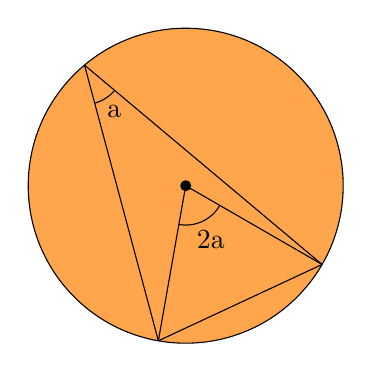
\begin{tikzpicture}[scale=2]
    %mark points on circle
        \coordinate[] (O) at (0,0);
        \coordinate[] (A) at (130:1);
        \coordinate[] (B) at (-30:1);
        \coordinate[] (E) at (260:1);

    %draw chords and circle
        \draw[name path=circ, fill = orange!70] (0,0) circle (1);
        \fill[black] (0,0) circle (1pt);
        \draw (B) -- (O);
        \draw (O) -- (E);
        \draw (A) -- (B);
        \draw (A) -- (E);
        \draw (E) -- (B);
      
        \pic [draw, "2a", angle eccentricity=1.5, angle radius = 0.5cm] {angle = E--O--B};
        \pic [draw, "a", angle eccentricity=1.4, angle radius = 0.5cm] {angle = E--A--B};
        
    \end{tikzpicture}

%5
    \begin{tikzpicture}[scale=2]
    % mark points on circle
        \coordinate[] (E) at (0,0);
        \coordinate[] (C) at (-45:1);
        \coordinate[] (A) at (150:1);
        \coordinate[] (B) at (40:1);
        \coordinate[] (D) at (230:1);

    % draw chords and circle
        \draw[name path=circ, fill=secondaryBlue] (0,0) circle (1);
        \draw[fill=secondaryBlue!50] (A) -- (B) -- (C) -- (D) -- cycle;
    
    \pic [draw, "a", angle eccentricity=1.5, angle radius = 0.5cm] {angle = D--A--B};
    \pic [draw, "b", angle eccentricity=1.5, angle radius = 0.5cm] {angle = A--B--C};
    \pic [draw, "c", angle eccentricity=1.5, angle radius = 0.5cm] {angle = B--C--D};
    \pic [draw, "d", angle eccentricity=1.5, angle radius = 0.5cm] {angle = C--D--A};
        
    \end{tikzpicture}

%Q6
    \begin{tikzpicture}[scale=2]
    % mark points on circle
        \coordinate[] (D) at (-90:1);

    % draw chords and circle
        \draw[name path=circ] (0,0) circle (1);

    % draw tangent
        \draw (D) -- ($(D)!1.5!-90:(0,0)$) coordinate (L) coordinate[pos = 0.1, yshift= 0.2cm] (P);
        \draw (D) -- ($(D)!1.5!90:(0,0)$) coordinate (E);

    % 
        \path[name path=DB] (D) -- ($(D)!1.5!-30:(E)$);
        \path[name path=DA] (D) -- ($(D)!2!-15:(0,0)$);
        \path[name intersections={of=DB and circ, by={B}}];
        \path[name intersections={of=DA and circ, by={A,temp}}];

    %Draw Chords
    \draw (D) -- (B);
    \draw (A) -- (D) coordinate[pos=0.3] (J);
    \draw (A) -- (B) coordinate[pos=0.9, yshift = -0.2cm] (M);

    %fill segment
    \filldraw[fill=lightRed!40] 
     (A) -- (D)
      arc[start angle=-90, end angle=45, radius=1cm]
      -- cycle;


    %Label Diagram %UNCOMMENT TO REMOVE LABELS
    \draw (J) -- ++(30:0.8cm) node[anchor = west] (K) {Chord};
    \draw (M) -- ++(-150:0.4cm) node[anchor = east, align = center] (N) {Angle in the \\ opposite segment};
    \draw (P) -- ++(20:0.8cm) node[anchor = west, align = center] (Q) {Angle between \\ tangent and chord};
    
    
    \pic [draw, "b", angle eccentricity=1.3, angle radius = 0.6cm] {angle = L--D--A};
    \pic [draw, "b", angle eccentricity=1.3, angle radius = 0.6cm] {angle = D--B--A};
        
    \end{tikzpicture}

%7
    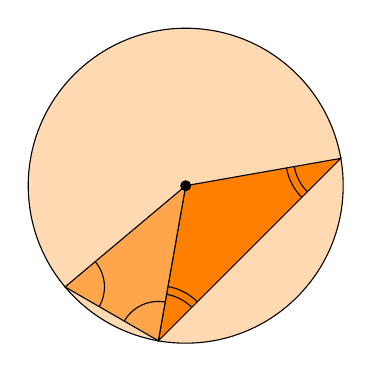
\begin{tikzpicture}[scale=2]
    %mark points on circle
        \coordinate[] (O) at (0,0);
        \coordinate[] (A) at (220:1);
        \coordinate[] (B) at (10:1);
        \coordinate[] (E) at (260:1);

    %draw chords and circle
        \draw[name path=circ, fill = orange!30] (0,0) circle (1);
        \draw[fill= orange] (B) -- (O) -- (E) -- cycle;
        \draw[fill = orange!70] (A) -- (O) -- (E) -- cycle;
        \fill[black] (0,0) circle (1pt);
      
        \pic [draw, angle eccentricity=1.5, angle radius = 0.6cm] {angle = B--E--O};
        \pic [draw,angle eccentricity=1.4, angle radius = 0.6cm] {angle = O--B--E};
        \pic [draw, angle eccentricity=1.5, angle radius = 0.7cm] {angle = B--E--O};
        \pic [draw,angle eccentricity=1.4, angle radius = 0.7cm] {angle = O--B--E};
        \pic [draw, angle eccentricity=1.5, angle radius = 0.5cm] {angle = E--A--O};
        \pic [draw,angle eccentricity=1.4, angle radius = 0.5cm] {angle = O--E--A};
        
    \end{tikzpicture}
%Q8
    \begin{tikzpicture}[scale=2]
    % mark points on circle
        \coordinate[] (D) at (0,0);
        \coordinate[] (A) at (-90:1);

    % draw chords and circle
        \draw[name path=circ, fill=primaryBlue!70] (0,0) circle (1);
        \fill[black] (0,0) circle (1pt);
        \draw (D) -- (A) coordinate[pos = 0.3, label = right:Radius];
        
    % draw tangent
    \draw (A) -- ($(A)!1.5!-90:(D)$) coordinate (L);
    \draw (A) -- ($(A)!1.5!90:(D)$) coordinate (M) coordinate[pos=0.3, label=below:Tangent];

    %marking right angles
    \tkzMarkRightAngle[size=.2](D,A,M);
        
    \end{tikzpicture}
 
%9
    \begin{tikzpicture}[scale=2]
    %mark points on circle
        \coordinate[] (O) at (0,0);
        \coordinate[] (B) at (-10:1);
        \coordinate[] (E) at (260:1);

    %draw chords and circle
        \draw[name path=circ, fill = lightYellow] (0,0) circle (1);
        \draw (O) -- ++(-55:1) coordinate[pos = 0.3] (J);
        \draw(B)  -- (E) coordinate[pos=0.5] (K) coordinate[pos=0.4] (Q);
        \fill[black] (0,0) circle (1pt);

        %label center
        \node[anchor = south west] at (O) {$O$};

        %marking right angles
        \tkzMarkRightAngle[size=.2](O,K,E);
        %marking congruent segments
        \tkzMarkSegment[pos=.5,mark=||](K,E);
        \tkzMarkSegment[pos=.5,mark=||](K,B);

        %arrow labels
        \draw [-Stealth] (0.5,0.5)  node[above] {Perpendicular bisector} -- (J);
        \draw [-Stealth] (1.1, -0.6)  node[right] {Chord} -- (Q);
        
    \end{tikzpicture}
\end{document}
